\section{Critical Context}

A CNN is a class of artificial neural network, or simply neural network, having a basic unit known as a neuron, a mathematical model developed by McCulloch and Pitts (1943), based on biological models of the human brain. Neurons are defined as real numbers, in the form of weighted inputs and a bias, and an activation function, which, given a sum of input values multiplied by weights, plus the bias, generates an output value. The combination of weights and bias represents an encoding, the biological equivalent being a memory. 

Based on the McCulloch-Pitts neuron, Donald Hebb (1949) created the first learning algorithm, that enables a neural network consisting of one single neuron to "learn", or encode, a memory, through an iteration process until, given a cost (or error) function, a set of weights and bias is found such that the same desired output is produced after a number of iterations, and the weights and bias reach stable values while the error is minimized. The Hebbian learning algorithm was able to learn simple tasks such as how to compute the OR truth table, but not more complex tasks such as the XOR truth table. This hindrance is known as a linear separability problem, where, using the inputs as coordinates, the output classes (0,1) of the XOR truth table plotted on a Cartesian plane, cannot be separated by a straight line. Solutions were eventually found, one involving the addition of another layer containing one neuron, known as a "hidden" layer, plus a connection between neurons, plus connections between inputs and the hidden layer neuron. The intuition being, a neural network with more neurons and more connections is able to learn more complex tasks. Such neural network architectures are known as multi-layer perceptrons (MLP) (\cite{Garcez}).  
In the model previously described, inputs are multiplied by weights. In the CNN model, inputs are "convolved" with weights. The concept is borrowed from the digital signal processing domain, where a vector known as a filter or kernel, is combined with a signal to generate a filtered output signal. The operation is expressed by:
\begin{equation}
\label{eqn:1dconv}
conv(s1,s2)[t1]=\sum_{t=0}^{N2-1} s1[t1-t]s2[t]    
\end{equation}
where $s1$ is the input signal, $s2$ is the kernel, $N2$ is the length of $s2$ and $t1$ is the time when input signal $s1$ was acquired. Convolution is similar to cross-correlation (where a measure of similarity between two signals is obtained) except convolution involves "flipping" one of the inputs. This can be observed by the indexing in $s1[t1-t]$ (\cite{Pauwels}). 

For the case of a two-dimensional input and kernel, the operation takes the form:

\begin{equation}
J(x,y) = K * I = \sum_{n,m}K(n,m)I(x-n,y-m) 
\end{equation}
Where $J$ is the convolved signal, $K$ is the kernel, $I$ is the input signal, and $n,m$ are the kernel indexes. We see by the input signal indexing $I(x-n,y-m)$ that both input signal axes are "flipped".

A typical CNN architecture will have a number of convolutional layers, following by a fully connected MLP, that is, where every neuron is connected to each other. The convolutional layers are able to compress the input, without losing discriminative information, into a lower dimensional space, where different input categories can be efficiently represented.
The fully-connected MLP layers then perform classification. Convolutional layers in neural networks with the ability to "self-organize", were introduced by the neocognitron network, proposed by \cite{fukushima:neocognitronbc}, particularly efficient for image pattern recognition.

Finding optimal weights and biases for a neural network in a large search space is a mathematically intractable problem that can be solved by the use of back-propagation and gradient descent algorithms, like proposed by \cite{Rumelhart:1986we} and \cite{Lecun98gradient-basedlearning}, which lead to the wide adoption of CNNs.

The concepts described have been implemented in several machine learning libraries such as Facebook's PyTorch, Google's Tensorflow and MATLAB toolkits. Designing a network from scratch can amount in some cases to writing a few lines of code.  

Self-driving vehicles have generally relied on designs where various sensor inputs are combined to generate a control signal (\cite{3899}) such as the pioneering Autonomous Land Vehicle (ALV) (Figure \ref{fig:alv_system_configuration}) . The ALV computer vision system, Vision Task Sequencer (VITS), treats the task of identifying the road ahead as a general classification problem with each pixel in any given image belonging to one of two classes, road and non-road. This is achieved by feature extraction, clustering and segmentation. Feature extraction is the process of engineering features that allow classes to be distinguished. Clustering partitions the feature space into mutually exclusive regions and segmentation assigns each image pixel to one regions The goal being to define regions that can be separated by a hyperplane (with dimension of the feature space minus one) boundary. Colour is used as the feature space. Other image features such as texture, saturation and reflectance from the laser scanner were not used.
\begin{figure}[ht]
 \centering 
 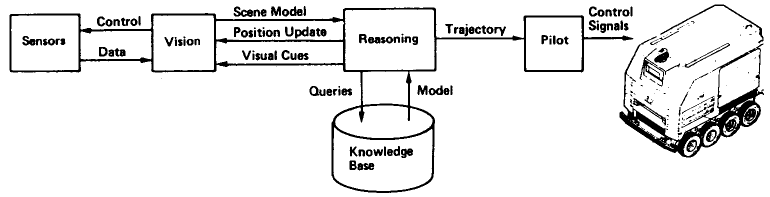
\includegraphics[width=\columnwidth]{figures/ALV-system-configuration.png}
 \caption{The ALV system configuration}
 \label{fig:alv_system_configuration}
\end{figure}

Back-propagation was used to train the neural network for the next-generation ALV, the ALVINN, Autonomous Land Vehicle In a Neural Network (\cite{NIPS1988_95}),  which has a 3-layer network designed for the task of road following, taking images from a camera and a laser range finder (such as lidar) as input and producing the direction the vehicle should travel in order to follow the road as output. The neural network architecture consists of 30x32 video inputs, 8x32 laser range finder inputs 29 hidden units, one road intensity feedback unit and 45 direction output units. The road intensity feedback unit indicates whether the road is lighter or darker
than the non-road in the previous image. The network is fully connected, that is, each of the input units is fully connected to the hidden layer, and each unit of the hidden layer is fully connected to the output layer.
These improvements eventually lead to the RALPH system, used for a self-driving vehicle that in 1995 drove almost entirely autonomously across the USA.

The NVIDIA CNN (Figure \ref{fig:nvidia_cnn}) maps raw pixels from a single front-facing camera directly to steering commands. (\cite{journals/corr/BojarskiTDFFGJM16}). A CNN image-in, steering-out had been previously implemented in a sub-scale radio control (RC) vehicle by the Defense Advanced Research Project Agency (DARPA) Autonomous Vehicle (DAVE) project. The end to end approach avoids the need for manual feature-extraction, clustering, segmentation and rules-based programming used to combined inputs and generate an output.


\begin{figure}[ht]
 \centering 
 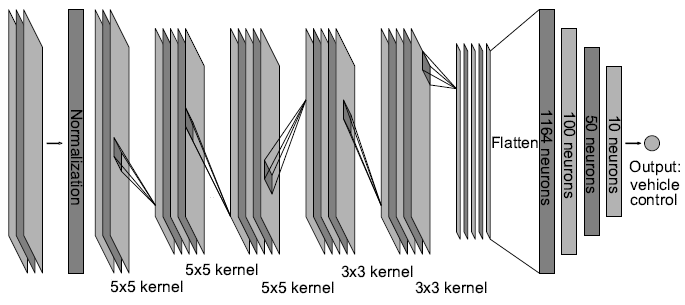
\includegraphics[width=\columnwidth]{figures/nvidia-end-to-end-horizontal.png}
 \caption{NVIDIA End-to-End CNN architecture}
 \label{fig:nvidia_cnn}
\end{figure}

The NVIDIA CNN has approximately 27 million connections and 250 thousand parameters. The network consists of 9 layers, including a normalization layer, 5 convolutional layers and 3 fully connected layers leading to an output control value which is the inverse of the turning radius $\frac{1}{r}$ to avoid a singularity when driving straight (infinite radius).
To remove a bias towards driving straight, a higher proportion of frames representing curves were added to the training data. The data was also augmented by random rotations to teach the network how to recover from unexpected shifts.
The network runs on dedicated graphical processing units (GPU) hardware able to apply far more data and computational power to the task compared to previously used central processing units (CPU).
This is the baseline network we are aiming to implement as a starting point to our evaluation.




